% !TeX program = pdflatex
\documentclass[aspectratio=169]{beamer}
\usepackage{amsmath,tikz}
\usetheme{default}
\usecolortheme{dove}
\setbeamertemplate{navigation symbols}{}
\title{Shortest paths by relaxation}
\subtitle{A dynamic programming argument}
\author{}\date{}
\begin{document}
\begin{frame}
\titlepage
\end{frame}
\begin{frame}{Relaxation}
\begin{figure}
\centering
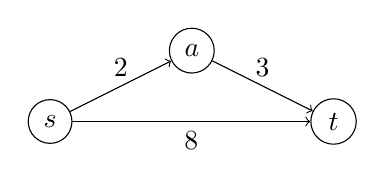
\begin{tikzpicture}[scale=0.9]
\node[draw,circle] (s) at (0,0) {$s$};
\node[draw,circle] (a) at (2,1) {$a$};
\node[draw,circle] (t) at (4,0) {$t$};
\draw[->] (s)--node[above]{$2$}(a);
\draw[->] (a)--node[above]{$3$}(t);
\draw[->] (s)--node[below]{$8$}(t);
\end{tikzpicture}
\end{figure}
\pause
$d_0(s)=0$ and $d_0(v)=\infty$ for $v\ne s$.
\[d_k(v)=\min\left\{d_{k-1}(v),\min_{(u,v)\in E}
[d_{k-1}(u)+w(u,v)]\right\}.\]
\note{Compare the direct cost 8 with the two-edge cost 2+3=5.}
\end{frame}
\begin{frame}{Convergence}
\Large
Without a reachable negative cycle, a shortest path can be simple.
It uses at most $|V|-1$ edges.
\note{State the negative-cycle assumption before the stopping bound.}
\end{frame}
\begin{frame}{Path invariant}
\Large
After $k$ synchronous rounds, $d_k(v)$ is the minimum weight
of an $s$--$v$ walk with at most $k$ edges.
\end{frame}
\end{document}
